% Options for packages loaded elsewhere
\PassOptionsToPackage{unicode}{hyperref}
\PassOptionsToPackage{hyphens}{url}
%
\documentclass[
]{article}
\usepackage{amsmath,amssymb}
\usepackage{lmodern}
\usepackage{iftex}
\ifPDFTeX
  \usepackage[T1]{fontenc}
  \usepackage[utf8]{inputenc}
  \usepackage{textcomp} % provide euro and other symbols
\else % if luatex or xetex
  \usepackage{unicode-math}
  \defaultfontfeatures{Scale=MatchLowercase}
  \defaultfontfeatures[\rmfamily]{Ligatures=TeX,Scale=1}
\fi
% Use upquote if available, for straight quotes in verbatim environments
\IfFileExists{upquote.sty}{\usepackage{upquote}}{}
\IfFileExists{microtype.sty}{% use microtype if available
  \usepackage[]{microtype}
  \UseMicrotypeSet[protrusion]{basicmath} % disable protrusion for tt fonts
}{}
\makeatletter
\@ifundefined{KOMAClassName}{% if non-KOMA class
  \IfFileExists{parskip.sty}{%
    \usepackage{parskip}
  }{% else
    \setlength{\parindent}{0pt}
    \setlength{\parskip}{6pt plus 2pt minus 1pt}}
}{% if KOMA class
  \KOMAoptions{parskip=half}}
\makeatother
\usepackage{xcolor}
\usepackage[margin=1in]{geometry}
\usepackage{color}
\usepackage{fancyvrb}
\newcommand{\VerbBar}{|}
\newcommand{\VERB}{\Verb[commandchars=\\\{\}]}
\DefineVerbatimEnvironment{Highlighting}{Verbatim}{commandchars=\\\{\}}
% Add ',fontsize=\small' for more characters per line
\usepackage{framed}
\definecolor{shadecolor}{RGB}{248,248,248}
\newenvironment{Shaded}{\begin{snugshade}}{\end{snugshade}}
\newcommand{\AlertTok}[1]{\textcolor[rgb]{0.94,0.16,0.16}{#1}}
\newcommand{\AnnotationTok}[1]{\textcolor[rgb]{0.56,0.35,0.01}{\textbf{\textit{#1}}}}
\newcommand{\AttributeTok}[1]{\textcolor[rgb]{0.77,0.63,0.00}{#1}}
\newcommand{\BaseNTok}[1]{\textcolor[rgb]{0.00,0.00,0.81}{#1}}
\newcommand{\BuiltInTok}[1]{#1}
\newcommand{\CharTok}[1]{\textcolor[rgb]{0.31,0.60,0.02}{#1}}
\newcommand{\CommentTok}[1]{\textcolor[rgb]{0.56,0.35,0.01}{\textit{#1}}}
\newcommand{\CommentVarTok}[1]{\textcolor[rgb]{0.56,0.35,0.01}{\textbf{\textit{#1}}}}
\newcommand{\ConstantTok}[1]{\textcolor[rgb]{0.00,0.00,0.00}{#1}}
\newcommand{\ControlFlowTok}[1]{\textcolor[rgb]{0.13,0.29,0.53}{\textbf{#1}}}
\newcommand{\DataTypeTok}[1]{\textcolor[rgb]{0.13,0.29,0.53}{#1}}
\newcommand{\DecValTok}[1]{\textcolor[rgb]{0.00,0.00,0.81}{#1}}
\newcommand{\DocumentationTok}[1]{\textcolor[rgb]{0.56,0.35,0.01}{\textbf{\textit{#1}}}}
\newcommand{\ErrorTok}[1]{\textcolor[rgb]{0.64,0.00,0.00}{\textbf{#1}}}
\newcommand{\ExtensionTok}[1]{#1}
\newcommand{\FloatTok}[1]{\textcolor[rgb]{0.00,0.00,0.81}{#1}}
\newcommand{\FunctionTok}[1]{\textcolor[rgb]{0.00,0.00,0.00}{#1}}
\newcommand{\ImportTok}[1]{#1}
\newcommand{\InformationTok}[1]{\textcolor[rgb]{0.56,0.35,0.01}{\textbf{\textit{#1}}}}
\newcommand{\KeywordTok}[1]{\textcolor[rgb]{0.13,0.29,0.53}{\textbf{#1}}}
\newcommand{\NormalTok}[1]{#1}
\newcommand{\OperatorTok}[1]{\textcolor[rgb]{0.81,0.36,0.00}{\textbf{#1}}}
\newcommand{\OtherTok}[1]{\textcolor[rgb]{0.56,0.35,0.01}{#1}}
\newcommand{\PreprocessorTok}[1]{\textcolor[rgb]{0.56,0.35,0.01}{\textit{#1}}}
\newcommand{\RegionMarkerTok}[1]{#1}
\newcommand{\SpecialCharTok}[1]{\textcolor[rgb]{0.00,0.00,0.00}{#1}}
\newcommand{\SpecialStringTok}[1]{\textcolor[rgb]{0.31,0.60,0.02}{#1}}
\newcommand{\StringTok}[1]{\textcolor[rgb]{0.31,0.60,0.02}{#1}}
\newcommand{\VariableTok}[1]{\textcolor[rgb]{0.00,0.00,0.00}{#1}}
\newcommand{\VerbatimStringTok}[1]{\textcolor[rgb]{0.31,0.60,0.02}{#1}}
\newcommand{\WarningTok}[1]{\textcolor[rgb]{0.56,0.35,0.01}{\textbf{\textit{#1}}}}
\usepackage{graphicx}
\makeatletter
\def\maxwidth{\ifdim\Gin@nat@width>\linewidth\linewidth\else\Gin@nat@width\fi}
\def\maxheight{\ifdim\Gin@nat@height>\textheight\textheight\else\Gin@nat@height\fi}
\makeatother
% Scale images if necessary, so that they will not overflow the page
% margins by default, and it is still possible to overwrite the defaults
% using explicit options in \includegraphics[width, height, ...]{}
\setkeys{Gin}{width=\maxwidth,height=\maxheight,keepaspectratio}
% Set default figure placement to htbp
\makeatletter
\def\fps@figure{htbp}
\makeatother
\setlength{\emergencystretch}{3em} % prevent overfull lines
\providecommand{\tightlist}{%
  \setlength{\itemsep}{0pt}\setlength{\parskip}{0pt}}
\setcounter{secnumdepth}{5}
\ifLuaTeX
  \usepackage{selnolig}  % disable illegal ligatures
\fi
\IfFileExists{bookmark.sty}{\usepackage{bookmark}}{\usepackage{hyperref}}
\IfFileExists{xurl.sty}{\usepackage{xurl}}{} % add URL line breaks if available
\urlstyle{same} % disable monospaced font for URLs
\hypersetup{
  pdftitle={HUDM6122 Homework\_08},
  pdfauthor={Chenguang Pan},
  hidelinks,
  pdfcreator={LaTeX via pandoc}}

\title{HUDM6122 Homework\_08}
\author{Chenguang Pan}
\date{2023-04-22}

\begin{document}
\maketitle

\hypertarget{github-address}{%
\subsection{Github Address}\label{github-address}}

All my latest homework can be found on Github:
\url{https://github.com/cgpan/hudm6122_homeworks} . Thanks for checking
if interested.

\hypertarget{exercise-1}{%
\subsection{Exercise 1}\label{exercise-1}}

\emph{Do a correspondence analysis for the car-ratings (file cars.txt).
Explain how this table can be considered as a contingency table.The data
are averaged ratings for 24 car types from a sample of 40 persons. The
marks range from 1 (very good) to 6 (very bad).}

\textbf{MY SOLUTION:}

\begin{Shaded}
\begin{Highlighting}[]
\SpecialCharTok{\textgreater{}} \CommentTok{\# import the data}
\ErrorTok{\textgreater{}}\NormalTok{ df }\OtherTok{\textless{}{-}} \FunctionTok{read.table}\NormalTok{(}\StringTok{"cars.txt"}\NormalTok{, }\AttributeTok{header =}\NormalTok{ T)}
\SpecialCharTok{\textgreater{}} \FunctionTok{head}\NormalTok{(df)}
\NormalTok{     Type   Model Economy Service Long.run.Value Price Design SportyCar Safety}
\DecValTok{1}\NormalTok{    Audi     }\DecValTok{100}     \FloatTok{3.9}     \FloatTok{2.8}            \FloatTok{2.2}   \FloatTok{4.2}    \FloatTok{3.0}       \FloatTok{3.1}    \FloatTok{2.4}
\DecValTok{2}\NormalTok{     BMW 5series     }\FloatTok{4.8}     \FloatTok{1.6}            \FloatTok{1.9}   \FloatTok{5.0}    \FloatTok{2.0}       \FloatTok{2.5}    \FloatTok{1.6}
\DecValTok{3}\NormalTok{ Citroen      AX     }\FloatTok{3.0}     \FloatTok{3.8}            \FloatTok{3.8}   \FloatTok{2.7}    \FloatTok{4.0}       \FloatTok{4.4}    \FloatTok{4.0}
\DecValTok{4}\NormalTok{ Ferrari     N}\SpecialCharTok{/}\NormalTok{A     }\FloatTok{5.3}     \FloatTok{2.9}            \FloatTok{2.2}   \FloatTok{5.9}    \FloatTok{1.7}       \FloatTok{1.1}    \FloatTok{3.3}
\DecValTok{5}\NormalTok{    Fiat     Uno     }\FloatTok{2.1}     \FloatTok{3.9}            \FloatTok{4.0}   \FloatTok{2.6}    \FloatTok{4.5}       \FloatTok{4.4}    \FloatTok{4.4}
\DecValTok{6}\NormalTok{    Ford  Fiesta     }\FloatTok{2.3}     \FloatTok{3.1}            \FloatTok{3.4}   \FloatTok{2.6}    \FloatTok{3.2}       \FloatTok{3.3}    \FloatTok{3.6}
\NormalTok{  EasyHandling}
\DecValTok{1}          \FloatTok{2.8}
\DecValTok{2}          \FloatTok{2.8}
\DecValTok{3}          \FloatTok{2.6}
\DecValTok{4}          \FloatTok{4.3}
\DecValTok{5}          \FloatTok{2.2}
\DecValTok{6}          \FloatTok{2.8}
\end{Highlighting}
\end{Shaded}

This dataset is a two-way table that shows the values of different
attributes or characteristics (columns) for each type or model of a car
(rows). Each row represents a different car model and each column
represents a different attribute or characteristic of the car.
Therefore, it can be seen as a contingency table.

\begin{Shaded}
\begin{Highlighting}[]
\SpecialCharTok{\textgreater{}} \CommentTok{\# import the packages}
\ErrorTok{\textgreater{}} \FunctionTok{library}\NormalTok{(FactoMineR)}
\SpecialCharTok{\textgreater{}} \FunctionTok{library}\NormalTok{(factoextra)}
\SpecialCharTok{\textgreater{}} 
\ErrorTok{\textgreater{}} \CommentTok{\# combine the first two columns into one}
\ErrorTok{\textgreater{}}\NormalTok{ df[,}\DecValTok{1}\NormalTok{] }\OtherTok{\textless{}{-}} \FunctionTok{paste}\NormalTok{(df}\SpecialCharTok{$}\NormalTok{Type,df}\SpecialCharTok{$}\NormalTok{Model)}
\SpecialCharTok{\textgreater{}}\NormalTok{ df }\OtherTok{\textless{}{-}}\NormalTok{ df[,}\SpecialCharTok{{-}}\DecValTok{2}\NormalTok{]}
\SpecialCharTok{\textgreater{}} 
\ErrorTok{\textgreater{}} \CommentTok{\# write a function to calculate the chi{-}squared distance  }
\ErrorTok{\textgreater{}}\NormalTok{ D }\OtherTok{\textless{}{-}} \ControlFlowTok{function}\NormalTok{(x)\{}
\SpecialCharTok{+}\NormalTok{   a }\OtherTok{\textless{}{-}} \FunctionTok{t}\NormalTok{(}\FunctionTok{t}\NormalTok{(x)}\SpecialCharTok{/}\FunctionTok{colSums}\NormalTok{(x))}
\SpecialCharTok{+}\NormalTok{   ret }\OtherTok{\textless{}{-}} \FunctionTok{sqrt}\NormalTok{(}\FunctionTok{colSums}\NormalTok{((a[,}\FunctionTok{rep}\NormalTok{(}\DecValTok{1}\SpecialCharTok{:}\FunctionTok{ncol}\NormalTok{(x),}\FunctionTok{ncol}\NormalTok{(x))]}\SpecialCharTok{{-}} 
\SpecialCharTok{+}\NormalTok{                          a[,}\FunctionTok{rep}\NormalTok{(}\DecValTok{1}\SpecialCharTok{:}\FunctionTok{ncol}\NormalTok{(x),}\FunctionTok{rep}\NormalTok{(}\FunctionTok{ncol}\NormalTok{(x), }\FunctionTok{ncol}\NormalTok{(x)))])}\SpecialCharTok{\^{}}\DecValTok{2}\SpecialCharTok{*}
\SpecialCharTok{+}                         \FunctionTok{sum}\NormalTok{(x)}\SpecialCharTok{/}\FunctionTok{rowSums}\NormalTok{(x)))}
\SpecialCharTok{+}   \FunctionTok{matrix}\NormalTok{(ret, }\AttributeTok{ncol =} \FunctionTok{ncol}\NormalTok{(x))}
\SpecialCharTok{+}\NormalTok{ \}}
\SpecialCharTok{\textgreater{}} \CommentTok{\# chi{-}squared distance for columns}
\ErrorTok{\textgreater{}}\NormalTok{ dcols }\OtherTok{\textless{}{-}} \FunctionTok{D}\NormalTok{(df[,}\SpecialCharTok{{-}}\DecValTok{1}\NormalTok{])}
\SpecialCharTok{\textgreater{}}\NormalTok{ drows }\OtherTok{\textless{}{-}} \FunctionTok{D}\NormalTok{(}\FunctionTok{t}\NormalTok{(df[,}\SpecialCharTok{{-}}\DecValTok{1}\NormalTok{]))}
\SpecialCharTok{\textgreater{}} 
\ErrorTok{\textgreater{}} \CommentTok{\# run CA}
\ErrorTok{\textgreater{}}\NormalTok{ r1 }\OtherTok{\textless{}{-}} \FunctionTok{cmdscale}\NormalTok{(dcols, }\AttributeTok{eig=}\NormalTok{T)}
\SpecialCharTok{\textgreater{}}\NormalTok{ c1 }\OtherTok{\textless{}{-}} \FunctionTok{cmdscale}\NormalTok{(drows, }\AttributeTok{eig=}\NormalTok{T)}
\SpecialCharTok{\textgreater{}} \FunctionTok{plot}\NormalTok{(r1}\SpecialCharTok{$}\NormalTok{points, }\AttributeTok{xlim =} \FunctionTok{range}\NormalTok{(r1}\SpecialCharTok{$}\NormalTok{points[,}\DecValTok{1}\NormalTok{], c1}\SpecialCharTok{$}\NormalTok{points[,}\DecValTok{1}\NormalTok{]) }\SpecialCharTok{*} \FloatTok{1.5}\NormalTok{,}
\SpecialCharTok{+}      \AttributeTok{ylim =} \FunctionTok{range}\NormalTok{(r1}\SpecialCharTok{$}\NormalTok{points[,}\DecValTok{1}\NormalTok{], c1}\SpecialCharTok{$}\NormalTok{points[,}\DecValTok{1}\NormalTok{]) }\SpecialCharTok{*} \FloatTok{1.5}\NormalTok{, }\AttributeTok{type =} \StringTok{"n"}\NormalTok{,  }
\SpecialCharTok{+}      \AttributeTok{xlab =} \StringTok{"Coordinate 1"}\NormalTok{, }\AttributeTok{ylab =} \StringTok{"Coordinate 2"}\NormalTok{, }\AttributeTok{lwd =} \DecValTok{2}\NormalTok{)}
\SpecialCharTok{\textgreater{}} \FunctionTok{text}\NormalTok{(r1}\SpecialCharTok{$}\NormalTok{points, }\AttributeTok{labels =} \FunctionTok{colnames}\NormalTok{(df[,}\SpecialCharTok{{-}}\DecValTok{1}\NormalTok{]), }\AttributeTok{cex =} \FloatTok{0.3}\NormalTok{, }\AttributeTok{col=}\StringTok{"blue"}\NormalTok{)}
\SpecialCharTok{\textgreater{}} \FunctionTok{text}\NormalTok{(c1}\SpecialCharTok{$}\NormalTok{points, }\AttributeTok{labels =}\NormalTok{ df[,}\DecValTok{1}\NormalTok{], }\AttributeTok{cex =} \FloatTok{0.3}\NormalTok{)}
\end{Highlighting}
\end{Shaded}

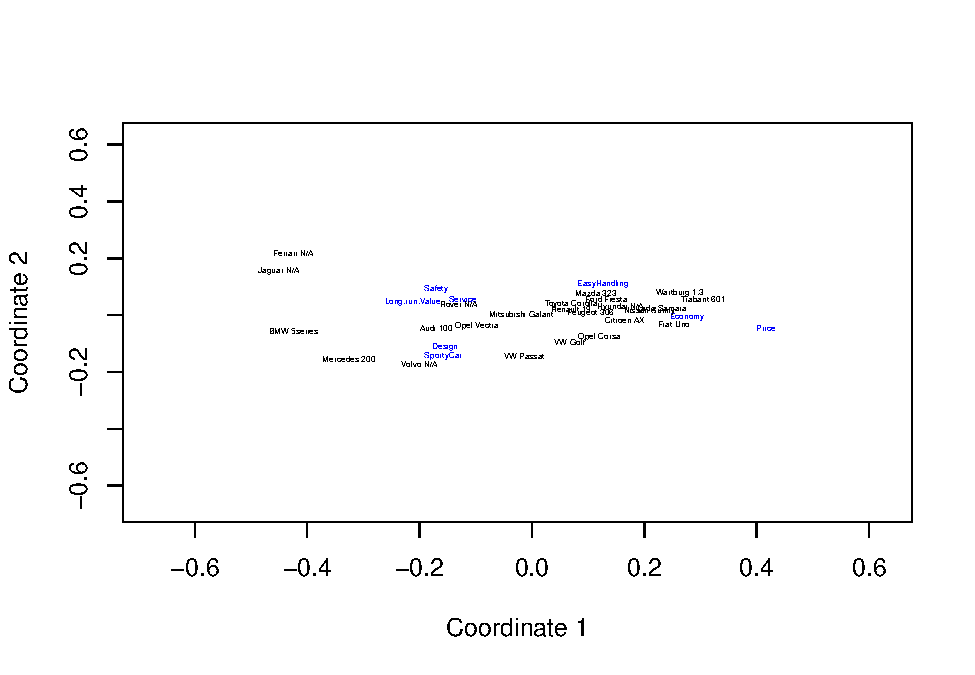
\includegraphics{HUDM6122-Homework_08-Chenguang-Pan_files/figure-latex/unnamed-chunk-2-1.pdf}

\hypertarget{exercise-2}{%
\subsection{Exercise 2}\label{exercise-2}}

\emph{Write an R function to compute the chi-square statistic of
independence. Test the null using for the bachelor data (file
bachelors.txt). The data consists of observations of 202,100 bachelors
from France and give the frequencies for different sets of modalities
classified into regions.}

\textbf{MY SOLUTION:}\\
Write the function first.

\begin{Shaded}
\begin{Highlighting}[]
\SpecialCharTok{\textgreater{}} \CommentTok{\# Function to compute chi{-}square statistic of independence}
\ErrorTok{\textgreater{}}\NormalTok{ chi\_square }\OtherTok{\textless{}{-}} \ControlFlowTok{function}\NormalTok{(table) \{}
\SpecialCharTok{+}   \CommentTok{\# Compute row and column totals}
\SpecialCharTok{+}\NormalTok{   row\_totals }\OtherTok{\textless{}{-}} \FunctionTok{apply}\NormalTok{(table, }\DecValTok{1}\NormalTok{, sum)}
\SpecialCharTok{+}\NormalTok{   col\_totals }\OtherTok{\textless{}{-}} \FunctionTok{apply}\NormalTok{(table, }\DecValTok{2}\NormalTok{, sum)}
\SpecialCharTok{+}\NormalTok{   n }\OtherTok{\textless{}{-}} \FunctionTok{sum}\NormalTok{(table) }\CommentTok{\# Total number of observations}
\SpecialCharTok{+}   
\SpecialCharTok{+}   \CommentTok{\# Compute expected values}
\SpecialCharTok{+}\NormalTok{   expected }\OtherTok{\textless{}{-}} \FunctionTok{outer}\NormalTok{(row\_totals, col\_totals) }\SpecialCharTok{/}\NormalTok{ n}
\SpecialCharTok{+}   
\SpecialCharTok{+}   \CommentTok{\# Compute chi{-}square statistic}
\SpecialCharTok{+}\NormalTok{   chi\_sq }\OtherTok{\textless{}{-}} \FunctionTok{sum}\NormalTok{((table }\SpecialCharTok{{-}}\NormalTok{ expected)}\SpecialCharTok{\^{}}\DecValTok{2} \SpecialCharTok{/}\NormalTok{ expected)}
\SpecialCharTok{+}   
\SpecialCharTok{+}   \CommentTok{\# Return result}
\SpecialCharTok{+}   \FunctionTok{return}\NormalTok{(chi\_sq)}
\SpecialCharTok{+}\NormalTok{ \}}
\end{Highlighting}
\end{Shaded}

Next, import the data and get the test.

\begin{Shaded}
\begin{Highlighting}[]
\SpecialCharTok{\textgreater{}} \CommentTok{\# import and clean the data}
\ErrorTok{\textgreater{}}\NormalTok{ df }\OtherTok{\textless{}{-}} \FunctionTok{read.table}\NormalTok{(}\StringTok{"bachelors.txt"}\NormalTok{, }\AttributeTok{header =}\NormalTok{ T)}
\SpecialCharTok{\textgreater{}} \FunctionTok{rownames}\NormalTok{(df) }\OtherTok{\textless{}{-}}\NormalTok{ df}\SpecialCharTok{$}\NormalTok{Abbrev.}
\SpecialCharTok{\textgreater{}}\NormalTok{ df }\OtherTok{\textless{}{-}}\NormalTok{ df[,}\SpecialCharTok{{-}}\FunctionTok{c}\NormalTok{(}\DecValTok{1}\NormalTok{,}\DecValTok{2}\NormalTok{,}\FunctionTok{ncol}\NormalTok{(df))]}
\SpecialCharTok{\textgreater{}} 
\ErrorTok{\textgreater{}} \CommentTok{\# run the function on this cleaned data}
\ErrorTok{\textgreater{}}\NormalTok{ (chi\_sq }\OtherTok{\textless{}{-}} \FunctionTok{chi\_square}\NormalTok{(df))}
\NormalTok{[}\DecValTok{1}\NormalTok{] }\FloatTok{4354.548}
\end{Highlighting}
\end{Shaded}

The function looks good. Next, get the pvalue.

\begin{Shaded}
\begin{Highlighting}[]
\SpecialCharTok{\textgreater{}} \CommentTok{\# get the degree of freedom}
\ErrorTok{\textgreater{}}\NormalTok{ dg\_fd }\OtherTok{\textless{}{-}}\NormalTok{ (}\FunctionTok{nrow}\NormalTok{(df) }\SpecialCharTok{{-}} \DecValTok{1}\NormalTok{) }\SpecialCharTok{*}\NormalTok{ (}\FunctionTok{ncol}\NormalTok{(df) }\SpecialCharTok{{-}} \DecValTok{1}\NormalTok{)}
\SpecialCharTok{\textgreater{}} \CommentTok{\# get the p{-}value}
\ErrorTok{\textgreater{}}\NormalTok{ (p\_value }\OtherTok{\textless{}{-}} \DecValTok{1} \SpecialCharTok{{-}} \FunctionTok{pchisq}\NormalTok{(chi\_sq, dg\_fd))}
\NormalTok{[}\DecValTok{1}\NormalTok{] }\DecValTok{0}
\end{Highlighting}
\end{Shaded}

Finally, compare the result with R-built-in function.

\begin{Shaded}
\begin{Highlighting}[]
\SpecialCharTok{\textgreater{}}\NormalTok{ test }\OtherTok{\textless{}{-}} \FunctionTok{chisq.test}\NormalTok{(df)}
\SpecialCharTok{\textgreater{}}\NormalTok{ test}

\NormalTok{    Pearson}\StringTok{\textquotesingle{}s Chi{-}squared test}

\StringTok{data:  df}
\StringTok{X{-}squared = 4354.5, df = 147, p{-}value \textless{} 2.2e{-}16}
\end{Highlighting}
\end{Shaded}

The results are identical.That is, we reject the null hypothesis. The
variables are not independent with each other!

\hypertarget{exercise-3}{%
\subsection{Exercise 3}\label{exercise-3}}

\emph{Do correspondence analysis of the U.S. crime data (file
UScrime.txt), and determine the absolute contributions for the first
three axes. How can you interpret the third axis? Try to identify the
states with one of the four regions to which it belongs. Do you think
the four regions have a different behavior with respect to crime?}

\textbf{MY SOLUTION:}

\begin{Shaded}
\begin{Highlighting}[]
\SpecialCharTok{\textgreater{}} \CommentTok{\# import the data}
\ErrorTok{\textgreater{}}\NormalTok{ df }\OtherTok{\textless{}{-}} \FunctionTok{read.table}\NormalTok{(}\StringTok{"UScrime{-}1.txt"}\NormalTok{, }\AttributeTok{header =}\NormalTok{ T)}
\SpecialCharTok{\textgreater{}} \FunctionTok{rownames}\NormalTok{(df) }\OtherTok{\textless{}{-}}\NormalTok{ df}\SpecialCharTok{$}\NormalTok{state}
\SpecialCharTok{\textgreater{}} \CommentTok{\# RUN CA}
\ErrorTok{\textgreater{}} \FunctionTok{library}\NormalTok{(FactoMineR)}
\SpecialCharTok{\textgreater{}}\NormalTok{ ca\_ }\OtherTok{\textless{}{-}} \FunctionTok{CA}\NormalTok{(df[}\DecValTok{4}\SpecialCharTok{:}\DecValTok{10}\NormalTok{], }\AttributeTok{graph =}\NormalTok{ F)}
\SpecialCharTok{\textgreater{}} \FunctionTok{summary}\NormalTok{(ca\_)}

\NormalTok{Call}\SpecialCharTok{:}
\FunctionTok{CA}\NormalTok{(}\AttributeTok{X =}\NormalTok{ df[}\DecValTok{4}\SpecialCharTok{:}\DecValTok{10}\NormalTok{], }\AttributeTok{graph =}\NormalTok{ F) }

\NormalTok{The chi square of independence between the two variables is equal to }\FloatTok{11287.55}\NormalTok{ (p}\SpecialCharTok{{-}}\AttributeTok{value =}  \DecValTok{0}\NormalTok{ ).}

\NormalTok{Eigenvalues}
\NormalTok{                       Dim}\FloatTok{.1}\NormalTok{   Dim}\FloatTok{.2}\NormalTok{   Dim}\FloatTok{.3}\NormalTok{   Dim}\FloatTok{.4}\NormalTok{   Dim}\FloatTok{.5}\NormalTok{   Dim}\FloatTok{.6}
\NormalTok{Variance               }\FloatTok{0.033}   \FloatTok{0.013}   \FloatTok{0.012}   \FloatTok{0.007}   \FloatTok{0.000}   \FloatTok{0.000}
\NormalTok{\% of var.             }\FloatTok{50.632}  \FloatTok{20.035}  \FloatTok{17.911}  \FloatTok{10.689}   \FloatTok{0.456}   \FloatTok{0.278}
\NormalTok{Cumulative \% of var.  }\FloatTok{50.632}  \FloatTok{70.667}  \FloatTok{88.577}  \FloatTok{99.266}  \FloatTok{99.722} \FloatTok{100.000}

\FunctionTok{Rows}\NormalTok{ (the }\DecValTok{10}\NormalTok{ first)}
\NormalTok{             Iner}\SpecialCharTok{*}\DecValTok{1000}\NormalTok{    Dim}\FloatTok{.1}\NormalTok{    ctr   cos2    Dim}\FloatTok{.2}\NormalTok{    ctr   cos2    Dim}\FloatTok{.3}
\NormalTok{ME         }\SpecialCharTok{|}     \FloatTok{0.335} \SpecialCharTok{|} \SpecialCharTok{{-}}\FloatTok{0.092}  \FloatTok{0.272}  \FloatTok{0.268} \SpecialCharTok{|}  \FloatTok{0.119}  \FloatTok{1.153}  \FloatTok{0.450} \SpecialCharTok{|} \SpecialCharTok{{-}}\FloatTok{0.091}
\NormalTok{NH         }\SpecialCharTok{|}     \FloatTok{0.415} \SpecialCharTok{|} \SpecialCharTok{{-}}\FloatTok{0.029}  \FloatTok{0.025}  \FloatTok{0.020} \SpecialCharTok{|}  \FloatTok{0.098}  \FloatTok{0.734}  \FloatTok{0.231} \SpecialCharTok{|} \SpecialCharTok{{-}}\FloatTok{0.174}
\NormalTok{VT         }\SpecialCharTok{|}     \FloatTok{1.094} \SpecialCharTok{|} \SpecialCharTok{{-}}\FloatTok{0.020}  \FloatTok{0.013}  \FloatTok{0.004} \SpecialCharTok{|}  \FloatTok{0.256}  \FloatTok{5.522}  \FloatTok{0.660} \SpecialCharTok{|} \SpecialCharTok{{-}}\FloatTok{0.167}
\NormalTok{MA         }\SpecialCharTok{|}     \FloatTok{4.467} \SpecialCharTok{|}  \FloatTok{0.324}  \FloatTok{6.895}  \FloatTok{0.510} \SpecialCharTok{|} \SpecialCharTok{{-}}\FloatTok{0.161}  \FloatTok{4.280}  \FloatTok{0.125} \SpecialCharTok{|} \SpecialCharTok{{-}}\FloatTok{0.252}
\NormalTok{RI         }\SpecialCharTok{|}     \FloatTok{2.489} \SpecialCharTok{|}  \FloatTok{0.126}  \FloatTok{1.177}  \FloatTok{0.156} \SpecialCharTok{|} \SpecialCharTok{{-}}\FloatTok{0.190}  \FloatTok{6.817}  \FloatTok{0.358} \SpecialCharTok{|} \SpecialCharTok{{-}}\FloatTok{0.169}
\NormalTok{CT         }\SpecialCharTok{|}     \FloatTok{0.649} \SpecialCharTok{|}  \FloatTok{0.089}  \FloatTok{0.481}  \FloatTok{0.245} \SpecialCharTok{|}  \FloatTok{0.001}  \FloatTok{0.000}  \FloatTok{0.000} \SpecialCharTok{|} \SpecialCharTok{{-}}\FloatTok{0.154}
\NormalTok{NY         }\SpecialCharTok{|}     \FloatTok{5.411} \SpecialCharTok{|}  \FloatTok{0.362} \FloatTok{11.019}  \FloatTok{0.673} \SpecialCharTok{|} \SpecialCharTok{{-}}\FloatTok{0.103}  \FloatTok{2.258}  \FloatTok{0.055} \SpecialCharTok{|}  \FloatTok{0.146}
\NormalTok{NJ         }\SpecialCharTok{|}     \FloatTok{1.175} \SpecialCharTok{|}  \FloatTok{0.201}  \FloatTok{2.521}  \FloatTok{0.709} \SpecialCharTok{|} \SpecialCharTok{{-}}\FloatTok{0.093}  \FloatTok{1.360}  \FloatTok{0.151} \SpecialCharTok{|} \SpecialCharTok{{-}}\FloatTok{0.067}
\NormalTok{PA         }\SpecialCharTok{|}     \FloatTok{8.652} \SpecialCharTok{|}  \FloatTok{1.124} \FloatTok{25.596}  \FloatTok{0.977} \SpecialCharTok{|}  \FloatTok{0.098}  \FloatTok{0.491}  \FloatTok{0.007} \SpecialCharTok{|} \SpecialCharTok{{-}}\FloatTok{0.129}
\NormalTok{OH         }\SpecialCharTok{|}     \FloatTok{0.389} \SpecialCharTok{|}  \FloatTok{0.069}  \FloatTok{0.297}  \FloatTok{0.253} \SpecialCharTok{|} \SpecialCharTok{{-}}\FloatTok{0.118}  \FloatTok{2.198}  \FloatTok{0.739} \SpecialCharTok{|}  \FloatTok{0.003}
\NormalTok{              ctr   cos2  }
\NormalTok{ME          }\FloatTok{0.762}  \FloatTok{0.266} \SpecialCharTok{|}
\NormalTok{NH          }\FloatTok{2.573}  \FloatTok{0.724} \SpecialCharTok{|}
\NormalTok{VT          }\FloatTok{2.613}  \FloatTok{0.279} \SpecialCharTok{|}
\NormalTok{MA         }\FloatTok{11.770}  \FloatTok{0.308} \SpecialCharTok{|}
\NormalTok{RI          }\FloatTok{6.050}  \FloatTok{0.284} \SpecialCharTok{|}
\NormalTok{CT          }\FloatTok{4.114}  \FloatTok{0.741} \SpecialCharTok{|}
\NormalTok{NY          }\FloatTok{5.066}  \FloatTok{0.109} \SpecialCharTok{|}
\NormalTok{NJ          }\FloatTok{0.801}  \FloatTok{0.080} \SpecialCharTok{|}
\NormalTok{PA          }\FloatTok{0.960}  \FloatTok{0.013} \SpecialCharTok{|}
\NormalTok{OH          }\FloatTok{0.002}  \FloatTok{0.001} \SpecialCharTok{|}

\NormalTok{Columns}
\NormalTok{             Iner}\SpecialCharTok{*}\DecValTok{1000}\NormalTok{    Dim}\FloatTok{.1}\NormalTok{    ctr   cos2    Dim}\FloatTok{.2}\NormalTok{    ctr   cos2    Dim}\FloatTok{.3}
\NormalTok{murder     }\SpecialCharTok{|}     \FloatTok{0.940} \SpecialCharTok{|}  \FloatTok{0.163}  \FloatTok{0.160}  \FloatTok{0.056} \SpecialCharTok{|}  \FloatTok{0.237}  \FloatTok{0.853}  \FloatTok{0.119} \SpecialCharTok{|}  \FloatTok{0.393}
\NormalTok{rape       }\SpecialCharTok{|}     \FloatTok{0.503} \SpecialCharTok{|}  \FloatTok{0.100}  \FloatTok{0.138}  \FloatTok{0.090} \SpecialCharTok{|}  \FloatTok{0.149}  \FloatTok{0.770}  \FloatTok{0.200} \SpecialCharTok{|}  \FloatTok{0.109}
\NormalTok{robbery    }\SpecialCharTok{|}    \FloatTok{14.193} \SpecialCharTok{|}  \FloatTok{0.486} \FloatTok{20.136}  \FloatTok{0.469} \SpecialCharTok{|} \SpecialCharTok{{-}}\FloatTok{0.220} \FloatTok{10.403}  \FloatTok{0.096} \SpecialCharTok{|}  \FloatTok{0.368}
\NormalTok{assault    }\SpecialCharTok{|}     \FloatTok{9.570} \SpecialCharTok{|}  \FloatTok{0.184}  \FloatTok{4.003}  \FloatTok{0.138} \SpecialCharTok{|}  \FloatTok{0.210} \FloatTok{13.213}  \FloatTok{0.180} \SpecialCharTok{|}  \FloatTok{0.326}
\NormalTok{burglary   }\SpecialCharTok{|}    \FloatTok{11.226} \SpecialCharTok{|}  \FloatTok{0.122} \FloatTok{11.952}  \FloatTok{0.352} \SpecialCharTok{|}  \FloatTok{0.138} \FloatTok{38.339}  \FloatTok{0.446} \SpecialCharTok{|} \SpecialCharTok{{-}}\FloatTok{0.079}
\NormalTok{larcery    }\SpecialCharTok{|}    \FloatTok{13.410} \SpecialCharTok{|} \SpecialCharTok{{-}}\FloatTok{0.151} \FloatTok{38.231}  \FloatTok{0.942} \SpecialCharTok{|} \SpecialCharTok{{-}}\FloatTok{0.033}  \FloatTok{4.737}  \FloatTok{0.046} \SpecialCharTok{|}  \FloatTok{0.017}
\NormalTok{auto.theft }\SpecialCharTok{|}    \FloatTok{15.402} \SpecialCharTok{|}  \FloatTok{0.281} \FloatTok{25.381}  \FloatTok{0.544} \SpecialCharTok{|} \SpecialCharTok{{-}}\FloatTok{0.197} \FloatTok{31.683}  \FloatTok{0.269} \SpecialCharTok{|} \SpecialCharTok{{-}}\FloatTok{0.121}
\NormalTok{              ctr   cos2  }
\NormalTok{murder      }\FloatTok{2.624}  \FloatTok{0.326} \SpecialCharTok{|}
\NormalTok{rape        }\FloatTok{0.461}  \FloatTok{0.107} \SpecialCharTok{|}
\NormalTok{robbery    }\FloatTok{32.689}  \FloatTok{0.269} \SpecialCharTok{|}
\NormalTok{assault    }\FloatTok{35.508}  \FloatTok{0.434} \SpecialCharTok{|}
\NormalTok{burglary   }\FloatTok{14.138}  \FloatTok{0.147} \SpecialCharTok{|}
\NormalTok{larcery     }\FloatTok{1.335}  \FloatTok{0.012} \SpecialCharTok{|}
\NormalTok{auto.theft }\FloatTok{13.244}  \FloatTok{0.100} \SpecialCharTok{|}
\ErrorTok{\textgreater{}} \CommentTok{\# table of eigenvalues}
\ErrorTok{\textgreater{}}\NormalTok{ row\_coord }\OtherTok{\textless{}{-}}\NormalTok{ ca\_}\SpecialCharTok{$}\NormalTok{row}\SpecialCharTok{$}\NormalTok{coord[,}\DecValTok{3}\NormalTok{]}
\SpecialCharTok{\textgreater{}}\NormalTok{ row\_coord[}\FunctionTok{order}\NormalTok{(row\_coord, }\AttributeTok{decreasing =} \ConstantTok{TRUE}\NormalTok{)[}\DecValTok{1}\SpecialCharTok{:}\DecValTok{7}\NormalTok{]]}
\NormalTok{       GA        MS        NC        MD        IL        NY        LA }
\FloatTok{0.3473941} \FloatTok{0.2309334} \FloatTok{0.2182393} \FloatTok{0.2081974} \FloatTok{0.1719769} \FloatTok{0.1461266} \FloatTok{0.1306424} 
\SpecialCharTok{\textgreater{}}\NormalTok{ ca\_}\SpecialCharTok{$}\NormalTok{col}\SpecialCharTok{$}\NormalTok{coord[,}\DecValTok{3}\NormalTok{]}
\NormalTok{     murder        rape     robbery     assault    burglary     larcery }
 \FloatTok{0.39332624}  \FloatTok{0.10927656}  \FloatTok{0.36809412}  \FloatTok{0.32560788} \SpecialCharTok{{-}}\FloatTok{0.07913001}  \FloatTok{0.01674929} 
\NormalTok{ auto.theft }
\SpecialCharTok{{-}}\FloatTok{0.12065495} 
\end{Highlighting}
\end{Shaded}

{[}Refer to Xue Yu's solution{]}\\
The absolute contributions for the first three axes are 50.63\%,
20.03\%, and 17.91\% respectively. The third axis can better represent
crimes related to personal injury (murder, robbery, and assault) in
states such as GA, MS, W, MD, etc.

\begin{Shaded}
\begin{Highlighting}[]
\SpecialCharTok{\textgreater{}} \FunctionTok{plot}\NormalTok{(ca\_, }\AttributeTok{col.row =}\NormalTok{ df}\SpecialCharTok{$}\NormalTok{region, }\AttributeTok{col.col=}\StringTok{"purple"}\NormalTok{)}
\end{Highlighting}
\end{Shaded}

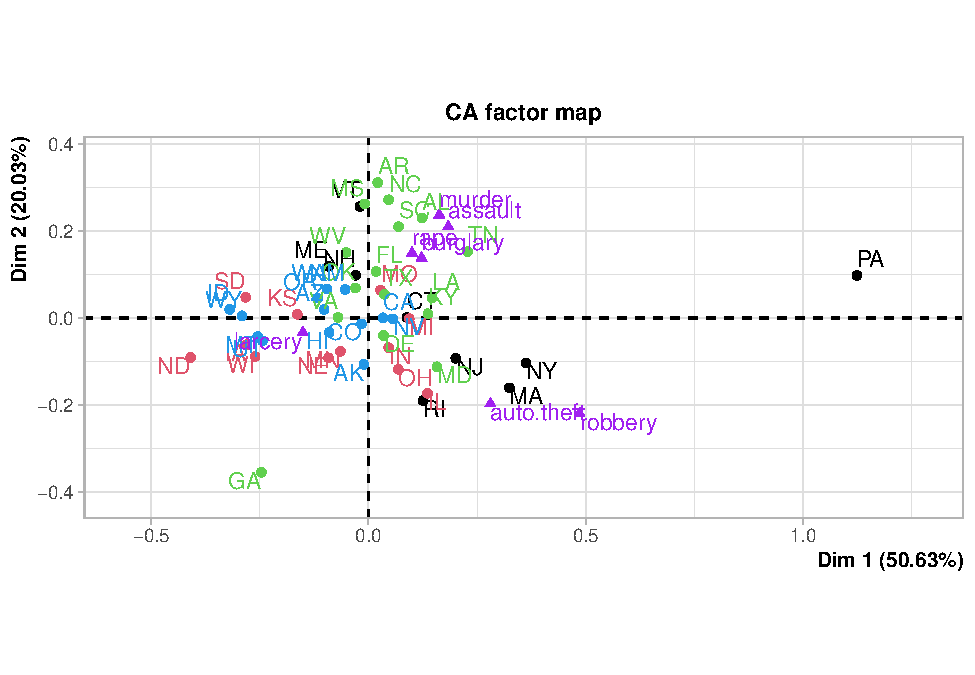
\includegraphics{HUDM6122-Homework_08-Chenguang-Pan_files/figure-latex/unnamed-chunk-8-1.pdf}
Northeast region (black points) is more related to auto.theft and
robbery. Some states in mid-west (red points), such as ND, IA, WI, and
SD are more related to larcery, while there are still some states in
mid-west, such as IN, OH,and IL are more related to auto.theft and
robbery. Most states from south (green points) are more related to roe,
burglary, murder and assault, Most states from west (blue points) are
more related to larcery.

\hypertarget{exercise-4}{%
\subsection{Exercise 4}\label{exercise-4}}

\emph{Consider the food data (file food.txt). Given that all of the
variables are measured in the same units (dollars), explain how this
table can be considered as a contingency table. Perform a correspondence
analysis and compare the results to those obtained with the PCA analysis
of the correlation matrix. The data set consists of the average
expenditures on food for several different types of families (manual
workers = MA, employees = EM, managers = CA) with different numbers of
children (2,3,4 or 5 children).}

\textbf{MY SOLUTION:}\\
Since the rows represent different workertypes and the columns represent
different food categories, and the values in the table can be seen as
the count or frequency of observations in each category for each
workertype, therefore this dataset can be considered as a contingency
table.

\begin{Shaded}
\begin{Highlighting}[]
\SpecialCharTok{\textgreater{}} \CommentTok{\# import the data}
\ErrorTok{\textgreater{}}\NormalTok{ df }\OtherTok{\textless{}{-}} \FunctionTok{read.table}\NormalTok{(}\StringTok{"food.txt"}\NormalTok{, }\AttributeTok{header =}\NormalTok{ T)}
\SpecialCharTok{\textgreater{}} \FunctionTok{rownames}\NormalTok{(df) }\OtherTok{\textless{}{-}}\NormalTok{ df}\SpecialCharTok{$}\NormalTok{Workertype}
\SpecialCharTok{\textgreater{}}\NormalTok{ df }\OtherTok{\textless{}{-}}\NormalTok{ df[,}\SpecialCharTok{{-}}\FunctionTok{c}\NormalTok{(}\DecValTok{1}\NormalTok{,}\DecValTok{2}\NormalTok{)]}
\SpecialCharTok{\textgreater{}} \FunctionTok{colnames}\NormalTok{(df)}
\NormalTok{[}\DecValTok{1}\NormalTok{] }\StringTok{"bread"}      \StringTok{"vegetables"} \StringTok{"fruits"}     \StringTok{"meat"}       \StringTok{"poultry"}   
\NormalTok{[}\DecValTok{6}\NormalTok{] }\StringTok{"milk"}       \StringTok{"wine"}      
\SpecialCharTok{\textgreater{}} \FunctionTok{dim}\NormalTok{(df)}
\NormalTok{[}\DecValTok{1}\NormalTok{] }\DecValTok{12}  \DecValTok{7}
\SpecialCharTok{\textgreater{}} \CommentTok{\# RUN CA}
\ErrorTok{\textgreater{}} \FunctionTok{library}\NormalTok{(FactoMineR)}
\SpecialCharTok{\textgreater{}}\NormalTok{ ca }\OtherTok{\textless{}{-}} \FunctionTok{CA}\NormalTok{(df,}\AttributeTok{graph=}\NormalTok{T)}
\end{Highlighting}
\end{Shaded}

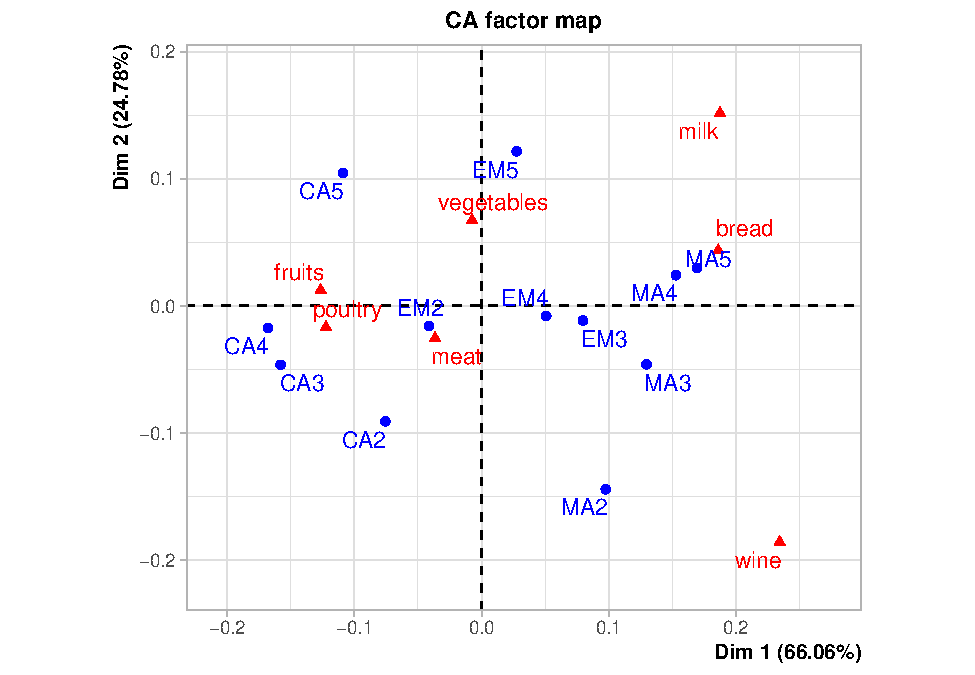
\includegraphics{HUDM6122-Homework_08-Chenguang-Pan_files/figure-latex/unnamed-chunk-9-1.pdf}

\begin{Shaded}
\begin{Highlighting}[]
\SpecialCharTok{\textgreater{}}\NormalTok{ ca}\SpecialCharTok{$}\NormalTok{eig}
\NormalTok{        eigenvalue percentage of variance cumulative percentage of variance}
\NormalTok{dim }\DecValTok{1} \FloatTok{0.0139275913}             \FloatTok{66.0607153}                          \FloatTok{66.06072}
\NormalTok{dim }\DecValTok{2} \FloatTok{0.0052247270}             \FloatTok{24.7816865}                          \FloatTok{90.84240}
\NormalTok{dim }\DecValTok{3} \FloatTok{0.0009972617}              \FloatTok{4.7301662}                          \FloatTok{95.57257}
\NormalTok{dim }\DecValTok{4} \FloatTok{0.0005210095}              \FloatTok{2.4712284}                          \FloatTok{98.04380}
\NormalTok{dim }\DecValTok{5} \FloatTok{0.0002978663}              \FloatTok{1.4128260}                          \FloatTok{99.45662}
\NormalTok{dim }\DecValTok{6} \FloatTok{0.0001145604}              \FloatTok{0.5433776}                         \FloatTok{100.00000}
\end{Highlighting}
\end{Shaded}

\begin{Shaded}
\begin{Highlighting}[]
\SpecialCharTok{\textgreater{}} \CommentTok{\# run PCA}
\ErrorTok{\textgreater{}}\NormalTok{ df\_scale }\OtherTok{\textless{}{-}} \FunctionTok{scale}\NormalTok{(df)}
\SpecialCharTok{\textgreater{}}\NormalTok{ pca }\OtherTok{\textless{}{-}} \FunctionTok{princomp}\NormalTok{(df, }\AttributeTok{cor=}\NormalTok{T)}
\SpecialCharTok{\textgreater{}} \FunctionTok{summary}\NormalTok{(pca)}
\NormalTok{Importance of components}\SpecialCharTok{:}
\NormalTok{                          Comp}\FloatTok{.1}\NormalTok{    Comp}\FloatTok{.2}\NormalTok{     Comp}\FloatTok{.3}\NormalTok{    Comp}\FloatTok{.4}\NormalTok{      Comp}\FloatTok{.5}
\NormalTok{Standard deviation     }\FloatTok{2.0816429} \FloatTok{1.3528822} \FloatTok{0.79425212} \FloatTok{0.3582283} \FloatTok{0.239908711}
\NormalTok{Proportion of Variance }\FloatTok{0.6190339} \FloatTok{0.2614700} \FloatTok{0.09011949} \FloatTok{0.0183325} \FloatTok{0.008222313}
\NormalTok{Cumulative Proportion  }\FloatTok{0.6190339} \FloatTok{0.8805039} \FloatTok{0.97062342} \FloatTok{0.9889559} \FloatTok{0.997178229}
\NormalTok{                            Comp}\FloatTok{.6}\NormalTok{       Comp}\FloatTok{.7}
\NormalTok{Standard deviation     }\FloatTok{0.137290211} \FloatTok{0.0300632132}
\NormalTok{Proportion of Variance }\FloatTok{0.002692657} \FloatTok{0.0001291138}
\NormalTok{Cumulative Proportion  }\FloatTok{0.999870886} \FloatTok{1.0000000000}
\end{Highlighting}
\end{Shaded}

I will choose the first two components to represent the data.

\begin{Shaded}
\begin{Highlighting}[]
\SpecialCharTok{\textgreater{}}\NormalTok{ xlim }\OtherTok{\textless{}{-}} \FunctionTok{range}\NormalTok{(pca}\SpecialCharTok{$}\NormalTok{scores[,}\DecValTok{1}\NormalTok{])}
\SpecialCharTok{\textgreater{}} \FunctionTok{plot}\NormalTok{(pca}\SpecialCharTok{$}\NormalTok{scores, }\AttributeTok{xlim=}\NormalTok{xlim, }\AttributeTok{ylim=}\NormalTok{xlim)}
\SpecialCharTok{\textgreater{}} \FunctionTok{text}\NormalTok{(pca}\SpecialCharTok{$}\NormalTok{scores, }\FunctionTok{rownames}\NormalTok{(df))}
\end{Highlighting}
\end{Shaded}

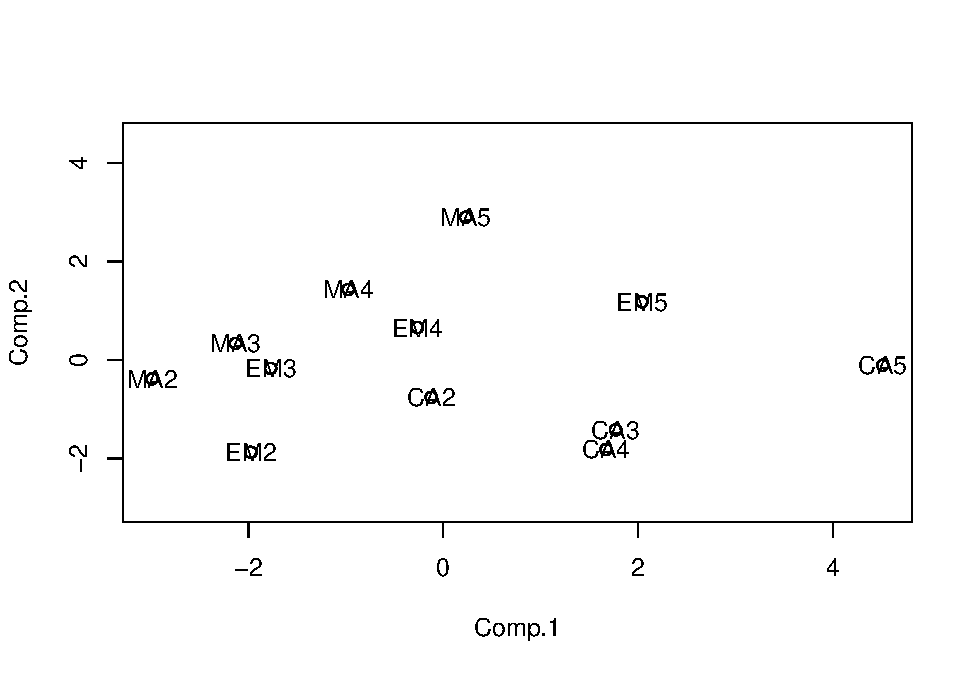
\includegraphics{HUDM6122-Homework_08-Chenguang-Pan_files/figure-latex/unnamed-chunk-11-1.pdf}

The two graphs show very similar results, since they all captures the
similarity between the workertypes, although the data points are shown
at different location.

\end{document}
